% Pre�mbulo del documento.
%-----------------------------------------------------------------%
% Clase de documento: libro
\documentclass[12pt,a4paper]{book} % article, report, book.

% Pre�mbulo: paquetes, comandos, entornos, estilos y t�tulo de p�gina.
%1 Codificaci�n e idioma%
\usepackage[latin1]{inputenc} %Codificaci�n en latin-1%
\usepackage[spanish]{babel}	%Hyphenation (Guionado) en espa�ol%
\usepackage[T1]{fontenc} %Codificaci�n de fuente%
\usepackage{eurofont} %Tipograf�a euro (�)%

%2 Matem�ticas y F�sica %
% Importante para ecuaciones, magnitudes y unidades%
\usepackage{amssymb,amsmath,latexsym,amsfonts} % paquetes est�ndar%
\usepackage[squaren]{SIunits} %Paquete para magnitudes y unidades f�sicas%
\usepackage{ifthen} %sentencias if y while%

%3 Gr�ficos%
\usepackage{graphics,graphicx} %paquetes gr�ficos est�ndar%
\usepackage{wrapfig} %paquete para gr�fica lateral%
\usepackage[rflt]{floatflt} %figuras flotantes%
	% \begin{floatingfigure}[r]/[l]{4.5cm}
	% \end{floatingfigure}
\usepackage{graphpap}	%comando \graphpaper en el entorno picture%

%4 Estilo y formato%
\usepackage{fancyhdr}	%cabeceras y pies mejor que con \pagestyle{}%
\usepackage{titlesec,titletoc} %Formateo de secciones y t�tulos%
\raggedbottom %Para fragmentar versos en varias p�ginas%
\usepackage{makeidx} %MakeIndex%
%\usepackage{showidx} % Hace que cada comando \index se imprima en la p�gina donde se ha puesto (�til para corregir los �ndices)
\usepackage{alltt} % Define el environment alltt, como verbatim, excepto que \, { y } tienen su significado normal. Se describe en el fichero alltt.dtx.
\usepackage[pdftex,bookmarksnumbered,hidelinks]{hyperref} %hyper-references%
\usepackage{minitoc} % Para poner tablas de contenido en cada cap�tulo.
\usepackage{listings} % Para escribir piezas de c�digo C, Python, etc. %
%listings configuration
\lstset{
  language=Python, %Puede ser C, C++, Java, etc.
  showstringspaces=false,
  formfeed=\newpage,
  tabsize=4,
  commentstyle=\itshape,
  basicstyle=\ttfamily,
  morekeywords={models, lambda, forms}
}

\usepackage{tipa} % tipograf�a IPA (International Phonetic Alphabet)
\usepackage{longtable} %Entorno Longtable, fracciona tablas a lo largo de p�ginas%
\usepackage{colortbl}
\usepackage{acronym}  %Para expandir autom�ticamente los acr�nimos
\usepackage{tikz}
\usepackage{pgf-umlsd}
\usepackage{url}
%%%%%%%%%%%%%%%%%%%%%%%%%%%%%%%%%%%%%%%%%%%%%%%%%%%%%%%%%%%%%%%%%%%
%%% Documento LaTeX 																						%%%
%%%%%%%%%%%%%%%%%%%%%%%%%%%%%%%%%%%%%%%%%%%%%%%%%%%%%%%%%%%%%%%%%%%
% T�tulo:	Comandos
% Autor:  Ignacio Moreno Doblas
% Fecha:  2014-02-01
%%%%%%%%%%%%%%%%%%%%%%%%%%%%%%%%%%%%%%%%%%%%%%%%%%%%%%%%%%%%%%%%%%%
% Tabla de materias:
% 1 Informaci�n del Documento %
% 2 Comandos a nivel de texto %
% 3 Comandos a nivel de entorno %
% 4 Comandos a nivel de p�gina y secci�n %
% 5 Otros comandos %
%%%%%%%%%%%%%%%%%%%%%%%%%%%%%%%%%%%%%%%%%%%%%%%%%%%%%%%%%%%%%%%%%%%

% 1 Informaci�n del Documento %
\newcommand{\pfctitlename}{T�tulo del Proyecto fin de Carrera}

\newcommand{\pfctitlenameenglish}{T�tulo del Proyecto fin de Carrera en Ingl�s}

\newcommand{\pfcauthorname}{Nombre del autor}
\newcommand{\pfctutorname}{Nombre del tutor}
\newcommand{\pfcanno}{a�o de publicaci�n}

% 2 Comandos a nivel de texto %
\newcommand{\R}{\textsuperscript{\textregistered}}	%S�mbolo registrado%
\newcommand{\C}{\textsuperscript{\copyright}}	%S�mbolo Copyright%
\newcommand{\TM}{\texttrademark} %S�mbolo Trade Mark (marca comercial)%

% 2.1 Comandos abreviatura %
\newcommand{\tit}{\textit} %Fuente cursiva (it�lica)%
\newcommand{\tbf}{\textbf} %Fuente negrita%
\newcommand{\ttw}[1]{\texttt{#1}} %Fuente m�quina de escribir (typewriter)%
%Combinaci�n%
\newcommand{\textittt}[1]{\textit{\texttt{#1}}} %it�lica y typewriter%
\newcommand{\textittw}{\textittt} % Otra forma de escribirlo.
\newcommand{\tittw}{\textittw} %Shortened%
\newcommand{\tbftw}[1]{\tbf{\ttw{#1}}}

%Crea una nueva l�nea y la indenta sin crear interlineado extra.
\newcommand{\nli}{\\ \indent} 

%Para escribir un correo electr�nico%
\newcommand{\mailto}[1]{\href{mailto:#1}{#1}}

% Si vas a hacer un uso b�sico de \index (entradas en el �ndice de s�lo un nivel, sin formatos especiales, etc.), define la orden
\newcommand{\miindex}[1]{#1\index{#1}}

\newcommand{\hs}{\hspace} % Abreviatura espacio horizontal
\newcommand{\vs}{\vspace} % Abreviatura espacio vertical

% Abreviaturas para los conjuntos de n�meros m�s comunes.
\newcommand{\realnumbers}{\mathbb R}
\newcommand{\naturalnumbers}{\mathbb N}
\newcommand{\integernumbers}{\mathbb Z}
\newcommand{\rationalnumbers}{\mathbb Q}
\newcommand{\complexnumbers}{\mathbb R}
\newcommand{\irrationalnumbers}{\mathbb I}

% Doble barra sobre una letra (para expresar las matrices).
\newcommand{\doublebar}[1]{\bar{\bar{#1}}} 
% Ej: \vector(y) = \doublebar(A) \vector(x) (Stma. lineal de ec.)

% 3 Comandos a nivel de entorno %
\newcommand{\benu}{\begin{enu}} % Begin enumerate
\newcommand{\eenu}{\end{enu}} 	% End enumeration

%Comando para escribir c�digo Python
\newcommand{\code}[3]{
  %\hrulefill
  %\subsection*{#1}
  %\subsubsection{#1}
  \lstinputlisting{#2}
  %#1\\
  \begin{table}[h!]
  	\centering
  	\caption{#1}
  	\label{#3}
  \end{table}
  \vspace{2em}
}

% 4 Comandos a nivel de p�gina y secci�n %
%Crea p�gina en blanco
\newcommand{\blankpage}{\clearpage{\pagestyle{empty}\cleardoublepage}}

% Versi�n x del comando section: sin numeraci�n pero s� aparece en la tabla de contenidos.
\newcommand{\sectionx}[1]{
	\section*{#1}
	\addcontentsline{toc}{section}{#1}
}

% Versi�n y del comando section: sin numeraci�n y NO aparece en la tabla de contenidos.
\newcommand{\sectiony}[1]{
	\section*{#1}
}

% Versi�n x del comando chapter: sin numeraci�n pero s�  aparece en la tabla de contenidos.
\newcommand{\chapterx}[1]{
	\chapter*{#1}
	%\addcontentsline{toc}{chapter}{#1} %Caused by minitoc package%
	\addstarredchapter{#1} %For minitoc package%
}

% substituto del comando \chapter: incluye estilo de p�gina.
\newcommand{\chapterbegin}[1]%
	{%
		\pagestyle{fancy}
		\fancyhead[LE,RO]{\thepage}
		\fancyhead[LO]{Cap�tulo \thechapter. #1}
		%\fancyhead[RE]{Parte \thepart \rightmark} %
		\fancyhead[RE]{\nouppercase{\rightmark}} %
				
		\chapter{#1}
	}

% Versi�n x del comando \chapterbegin: sin numeraci�n y aparece en la tabla de contenidos.
\newcommand{\chapterbeginx}[1]%
	{%
		\pagestyle{fancy}
		\fancyhead[RO,LE]{\thepage}
		\fancyhead[RE,LO]{#1}
		%\fancyhead[LO]{Chapter \thechapter}
		%\fancyhead[RE]{Part \thepart} %
		
		\chapterx{#1}
	}

% substituto del comando \chapter: incluye estilo de p�gina.
\newcommand{\chapterAppenbegin}[1]%
{%
	\pagestyle{fancy}
	\fancyhead[RO,LE]{\thepage}
	\fancyhead[LO]{Ap�ndice \thechapter. #1}
	%\fancyhead[RE]{Parte \thepart \rightmark} %
	\fancyhead[RE]{\nouppercase{\rightmark}} %
	
	\chapter{#1}
}

%Fin de cap�tulo
\newcommand{\chapterend}{\pagestyle{empty}\cleardoublepage \thispagestyle{empty}}
%Si fuera un art�culo en lugar un libro, \clearpage en lugar de \cleardoublepage

% 5 Otros comandos %
%\let\Oldpart\part
%\newcommand{\parttitle}{}
%\renewcommand{part}[1]{\Oldpart{#1}\renewcommand{\parttitle}{#1}} %Header customization%

%Cambiar el t�tulo �ndice de cap�tulo a ``Contenido''.
\renewcommand{\mtctitle}{Contenido}

\dominitoc % Para tablas de contenidos por cap�tulo.

\addto{\captionsspanish}{
	\renewcommand{\listtablename}{�ndice de Tablas}
	\renewcommand{\tablename}{Tabla} } % Por ejemplo, modificar el nombre de 'Cuadro' a 'Tabla'.

\addto{\captionsspanish}{
	\renewcommand{\contentsname}{�ndice} }

\renewcommand{\lstlistingname}{Listado}

%Si se desea cambiar el tipo de letra a Arial
% por cualquier raz�n, descomentar las siguientes
% dos l�neas
%\renewcommand{\rmdefault}{phv} % Arial
%\renewcommand{\sfdefault}{phv} % Arial
	
%\addto{\captionsspanish}{
%	\renewcommand{\partname}{Fase} }

%\addto{\captionsspanish}{%
%    \renewcommand{\refname}{\vspace{-4.5ex}}} % Para que no aparezca el texto 'referencias' en la bibliograf�a.

% Modifica el interlineado
%\renewcommand{\baselinestretch}{1.5}
%%%%%%%%%%%%%%%%%%%%%%%%%%%%%%%%%%%%%%%%%%%%%%%%%%%%%%%%%%%%%%%%%%%
%%% Documento LaTeX 																						%%%
%%%%%%%%%%%%%%%%%%%%%%%%%%%%%%%%%%%%%%%%%%%%%%%%%%%%%%%%%%%%%%%%%%%
% T�tulo:	Entornos
% Autor:  Ignacio Moreno Doblas
% Fecha:  2014-02-01
%%%%%%%%%%%%%%%%%%%%%%%%%%%%%%%%%%%%%%%%%%%%%%%%%%%%%%%%%%%%%%%%%%%
% Tabla de materias:
%--------------------%
% 1 dobleindent
% 2 izqindent
% 3 dobleindentx
% 4 ite
% 5 descript
% 6 enu
% 7 itemization
% 8 sinopsis
%%%%%%%%%%%%%%%%%%%%%%%
% Para conocer los par�metros de dise�o de las listas, tales como
%  los m�rgenes izquierdo, derechos y los diferentes saltos,
%  v�ase el archivo ``List layout.png'' que acompa�a esta plantilla.
% As� se conocer� mejor c�mo adaptar un entorno seg�n los requisitos 
%  del usuario.

%%%%%%%%%%%%%%%%%%%%%%%
% Definici�n de longitudes para usar en los entornos:
%
% Normal parskip.
\newlength{\parskipenv}
\setlength{\parskipenv}{\parskip}

\newlength{\parindentenv}
\setlength{\parindentenv}{\parindent}
%%%%%%%%%%%%%%%%%%%%%%%

% 1 dobleindent
%El entorno dobleindent est� pensando para escribir p�rrafos con doble indentaci�n a cada lado.
%Tiene dos par�metros de entrada con las distancias medidas desde los m�rgenes de p�gina.

\newenvironment{dobleindent}[2]
	%Comienzo de nuevo entorno%
	{
	\begin{list}
		{}
		{
		% Left and right margins:
		\leftmargin = #1 
		\rightmargin = #2
		%
		% Separation from preceding and following text:
		\topsep = 0ex
		\partopsep = 0ex
		\parsep = \parskipenv
		%
		% Indentation for paragraphs:
		\itemsep = \parskipenv
		\itemindent = \parindentenv
		\listparindent = \itemindent
		%
		% Horizontal separation from label:
		\labelsep = 1ex
		\settowidth{\labelwidth}{0cm}
		}
		
		 \item}
	% End new env
	{\end{list}}

%%%%%%%%%%%%%%%%%%%%%%%%%%%%%
%2 izqindent
% El entorno izqindent s�lo crea un p�rrafo indentado a la izquierda.
\newenvironment{izqindent}[1]
{
\begin{dobleindent}{#1}{0cm}
}
{
\end{dobleindent}
}

%%%%%%%%%%%%%%%%%%%%%%%%%%%%%
% 3 dobleindentx
% El entorno dobleindentx es una variaci�n del dobleindent usando leftskip y rightskip.
% Aunque es m�s limitado, tambi�n se puede usar.
\newenvironment{dobleindentx}[2] % S�lo funciona en modo paragraph
{ % Preamble
  \leftskip = #1
  \rightskip = #2
}
{ % Postamble
\leftskip = 0cm
\rightskip = 0cm
}

%%%%%%%%%%%%%%%%%%%%%%%%%%%%%
% 4 ite
% El entorno ite es una modificaci�n del entorno itemize est�ndar de \LaTeX. Puede usarse o modificarse si el usuario lo desea.
% Tambi�n puede parametrizarse el entorno enumerate o description de forma equivalente.
\newenvironment{ite}
	{
		\begin{izqindent}{\parindent}
		\hspace{-\parindent} 	% compensaci�n del sangrado que introduce el entorno.
		\vspace{-1.0\parskip}	% compensaci�n del \parskip que introduce el entorno.
		\vspace{-\baselineskip}	% compensaci�n por la l�nea que introduce el entorno.
		\begin{itemize}
	}
	{
		\end{itemize}
		\end{izqindent}
	}

%%%%%%%%%%%%%%%%%%%%%5
% commando stdformat para formatear los entornos descript, enu y itemization.
\newcommand{\stdformat}
	{% Declarations for format presentation.
		%		  
		% Separation from preceding and following text:
		\setlength{\topsep}{0ex}%
		\setlength{\partopsep}{0ex} %
		%
		% Horizontal separation from label:
		\labelsep = 1ex
		\setlength{\labelwidth}{0ex}
		%
		%	Left and right margins:	
		\setlength{\leftmargin}{1cm}%
		\addtolength{\leftmargin}{\labelsep}
		\setlength{\rightmargin}{0ex}
		%  
		% Indentation for paragraphs:
		\setlength{\itemindent}{-\leftmargin}%
		\addtolength{\itemindent}{1ex}
		\setlength{\listparindent}{\parindent}%
		%		
		% Separation between paragraphs.
		\setlength{\parsep}{\parskipenv}% 
		\setlength{\itemsep}{1ex}
	}

%%%%%%%%%%%%%%%%%%%%%%%%%%%%%
% 5 descript

\newenvironment{descript}
	% Beginning new env def.
	{
		\begin{list}
			{} % No default label for \item.
			{
				% Declarations for format presentation.
				\stdformat
				%
				\renewcommand{\makelabel}[1]{\normalfont\bfseries##1\hfil}
			}
	}
	% Ending new env def.
	{
		\hspace*{\fill} \\ \end{list}
	} % Se introduce un salto de l�nea para que el texto siguiente est� separado.
%END newenvironment{descript}

%%%%%%%%%%%%%%%%%%%%%%%%%%%%%
% 6 enu
\newcounter{itemnumber} % Counter for the environment.

\newenvironment{enu}
	% Beginning new env def.
	{
		\begin{list}
		{
			\raggedleft \arabic{itemnumber}
		}
		{
			\usecounter{itemnumber}
			\stdformat
		}
	}
	{
		\end{list}
	}

%%%%%%%%%%%%%%%%%%%%%%%%%%%%%
% 7 itemization
\newenvironment{itemization}
	% Beginning new env def.
	{
		\begin{list}
			{$\bullet$} % No default label for \item.
			{
				% Declarations for format presentation.
				\stdformat
			}
	}
	% Ending new env def.
	{
		\end{list}
	}


%%%%%%%%%%%%%%%%%%%%%%%%%%%%%
% 8 sinopsis
\newenvironment{sinopsis}{%[1]{
	\sectiony{Sinopsis}
	%\label{#1}
} {
	\pagebreak
}
%%%%%%%%%%%%%%%%%%%%%%%%%%%%%%%%%%%%%%%%%%%%%%%%%%%%%%%%%%%%%%%%%%%
%%% Documento LaTeX 																						%%%
%%%%%%%%%%%%%%%%%%%%%%%%%%%%%%%%%%%%%%%%%%%%%%%%%%%%%%%%%%%%%%%%%%%
% T�tulo:	Par�metros de estilo
% Autor:  Ignacio Moreno Doblas
% Fecha:  2014-02-01
%%%%%%%%%%%%%%%%%%%%%%%%%%%%%%%%%%%%%%%%%%%%%%%%%%%%%%%%%%%%%%%%%%%
% Tabla de materias:
%--------------------%
% 1 M�rgenes de p�gina
%%%%%%%%%%%%%%%%%%%%%%%
% Para conocer los par�metros de dise�o de p�ginas, tales como
%  los m�rgenes izquierdo, derecho, anchura de p�gina, etc.
%  v�ase el archivo ``Page layout.png'' que acompa�a esta plantilla.
% As� se conocer� mejor c�mo adaptar el documento seg�n los 
%  requisitos del usuario.

% 1 M�rgenes de p�gina
%-------------------------------%
% Par�metros de estilo de p�gina.
% DIN A4: 29.7 cm x 21 cm
%		�rea neta: 3 cm + 3 cm + 15 cm.
%
% Definici�n de m�rgenes de p�gina
%  even para p�ginas pares
%  odd  para p�ginas impares
\newlength{\realoddsidemargin}	  % \oddsidemargin menos 1 in.
\newlength{\realevensidemargin}		% \evensidemargin menos 1 in.
\newlength{\realtopmargin}				% \topmargin menos 1 in.
%
% Asignaci�n de m�rgenes de p�gina
% ASIGNESE en caso de querer cambiarlo
\setlength{\realtopmargin}{2cm}			% REAL top margin.
\setlength{\realoddsidemargin}{3cm}		% REAL oddside margin.
\setlength{\realevensidemargin}{3cm}	% REAL evenside margin.
\setlength{\hoffset}{0cm}
\setlength{\voffset}{0cm}
%
% Substracci�n de 1 pulgada de compensaci�n
%  (v�ase ``Page Layout.png'' para m�s informaci�n)
\addtolength{\realoddsidemargin}{-1in}	% 1 inch = 2.54 cm.
\addtolength{\realevensidemargin}{-1in}
\addtolength{\realtopmargin}{-1in}
%
% Asignaci�n de anchuras y m�rgenes
% No hay notas al margen
\setlength{\marginparsep}{0cm} % No van a existir notas al margen
\setlength{\marginparwidth}{0cm} % No van a existir notas al margen
%
% Asignaci�n de anchura de texto
\setlength{\textwidth}{15cm}	% Anchura neta del texto (globalmente).
%
% Asignaci�n de m�rgenes par, impar y en altura
\setlength{\oddsidemargin}{\realoddsidemargin}	% odd-page left margin (global).
\setlength{\evensidemargin}{\realoddsidemargin}	% even-page left margin (global).
\setlength{\topmargin}{\realtopmargin}					% top margin (Global).

% Se puede usar tambi�n el paquete chngpage.

%%%%%%%%%%%%%%%%%%%%%%%%%%%%%%%%%%%%%%%%%%%%%%%%%%%%%%%%%%%%%%%%%%
%		1 Length commands.					%
%-------------------------------%
% Defines new length command (e.g., \newlength{\gnat}}
%	\newlength{}
%
% Set lenght to a value.
%	\setlength{\gnat}{length}
%	\addtolength{}{}
%
% Sets the value of a length command equal to the width of a specified piece of text; e.g., \settowidth{\parindent}{\em small}.
%	\settowidth{}{}
% Set the value of a height. e.g., \settoheight{\parskip}{Gnu}
%	\settoheight{}{}
% Set the value that extends below the line. e.g., \settodepth{\parskip}{gnu}.
%	\settodepth{}{}
%
% To multiply a length, write: 7.0\gnat = \gnat * 7.0
%%%%%%%%%%%%%%%%%%%%%%%%%%%%%%%%%%%%%%%%%%%%%%%%%%%%%%%%%%%%%%%%%%

%Comando para crear glosario (index en ingl�s)
\makeindex


% Document body.
%-------------------------------------------------------------------%
\begin{document}

% Formato de documento hasta el cap�tulo 1 (sin incluirlo)
\frontmatter

%% T�tulo y autor del proyecto
%%Rellenar con el nombre real del autor, t�tulo, tutor y a�o.
%%El departamento del tutor se escribe una vez en el Resumen del PFC
\renewcommand{\pfcauthorname}{JOS� ANTONIO Y�BENES G�LVEZ}
\renewcommand{\pfctitlename}{Plataforma inal\'{a}mbrica para la web f�sica}
\renewcommand{\pfctutorname}{Ignacio Herrero y Jos� Manuel Cano}
\renewcommand{\pfcanno}{2017}

% Portada.
%%% Tipos de portada %%%
%	1. \maketitle
%	2. titlepage
%%%%%%%%%%%%%%%%%%%%%%%%

%	1. \maketitle
%%%%%%%%%%%%%%%%%%%%%%%%
%\maketitle
%\thispagestyle{empty}

%	2. titlepage
%%%%%%%%%%%%%%%%%%%%%%%%
\begin{titlepage}
	\begin{center}
		\Large{
		UNIVERSIDAD DE M�LAGA
		}
	\end{center}
	\begin{center}
		\Large {
		ESCUELA T�CNICA SUPERIOR DE \\
		INGENIER�A DE TELECOMUNICACI�N
		}
	\end{center}
	
	\vspace{30mm}
	
	\begin{center}\Large{TRABAJO DE FIN DE GRADO}\end{center}
	
	\vspace{20mm}
	
	\begin{center}
		\huge
		\sffamily\scshape
		\pfctitlename		
	\end{center}
	
	\vspace{20mm}
	
	\begin{center}
		\large
		\scshape%\bfseries
		\textsf{GRADO EN INGENIER�A DE \\ TECNOLOG�AS DE TELECOMUNICACI�N}
	\end{center}
	
	\vfill
	
	 \hfill \pfcauthorname  
	 
	 
	 \hfill M�LAGA, \pfcanno 
	 
	\blankpage
	
\end{titlepage}


% Hoja de calificaci�n
\thispagestyle{empty}
\begin{center}
	\Large \sffamily \scshape %\bfseries
	Escuela T�cnica Superior de\\
	Ingenier�a de Telecomunicaci�n\\
	Universidad de M�laga
\end{center}

	{\bfseries Titulaci�n: Grado en Ingenier�a de Tecnolog�as de Telecomunicaci�n}\\[3ex]

	\noindent Reunido el tribunal examinador en el d�a de la fecha, constituido por:\\[3ex]
	\textbf{D./D�.~}\hrulefill\\[3ex]
	\textbf{D./D�.~}\hrulefill\\[3ex]
	\textbf{D./D�.~}\hrulefill\\[3ex]
	
	para juzgar el Trabajo de Fin de Grado titulado:\noindent 
	
\begin{center}
	\large \bfseries \pfctitlename
\end{center}

\noindent del alumno \tit{D./D�.~\pfcauthorname}

\noindent dirigido por \tit{D./D�.~\pfctutorname}

\bigskip

	\noindent ACORD� POR \hrulefill OTORGAR LA\\[3ex]%\rule{3cm}{0.1mm} otorgar la\\[3ex]
	CALIFICACI�N DE\hrulefill\\[3ex]
	
	%\hrulefill\\[3ex]
	
	\noindent y, para que conste, se extiende firmada por los componentes del tribunal, la presente diligencia.
	
	\bigskip

\hfill M�laga, a \rule{1cm}{0.1mm} de \rule{1cm}{0.1mm} de \rule{0.7cm}{0.1mm}

\vfill

\begin{center}
	\begin{tabular}{ccc}
	El Presidente: & El Vocal: & El Secretario:\\[2cm]
	Fdo.:\rule{3cm}{0.1mm} & Fdo.:\rule{3cm}{0.1mm} & Fdo.:\rule{3cm}{0.1mm}	
	\end{tabular}
\end{center}

\blankpage

% Resumen del proyecto (formulario)
%%%%%%%%%%%%%%%%%%%%%%%%%%%%%%%%%%
% P�gina de resumen del proyecto %
%%%%%%%%%%%%%%%%%%%%%%%%%%%%%%%%%%

\thispagestyle{empty}
\begin{center}
	\Large \sffamily
	Universidad de M�laga\\
	Escuela T�cnica Superior de Ingenier�a de\\
	Telecomunicaci�n
\end{center}

\bigskip

\begin{center}
	\Huge\scshape
	\pfctitlename
\end{center}

\bigskip

\begin{center}
	\textbf{REALIZADO POR}\\
	\textsf{\pfcauthorname}
\end{center}

\medskip

\begin{center}
	\textbf{DIRIGIDO POR}\\
	\textsf{\pfctutorname}
\end{center}

\vfill

\begin{minipage}{\textwidth}
\textbf{Dpto. de:} Ingenier�a de Comunicaciones (DIC)

\medskip

\textbf{Palabras clave:} palabras, clave, del, proyecto, separadas, por, coma

\medskip

\textbf{Titulaci�n:} Ingenier�a de Telecomunicaci�n

\medskip

\textbf{Resumen:}
	Aqu� se explica un breve resumen del proyecto, en qu� consiste, cu�l es
su prop�sito, etc.\\
	Puede usarse m�s de un p�rrafo si es necesario.

\begin{center} M�laga, \today\end{center}
\end{minipage}

\blankpage

% Dedicatoria.
%%%%%%%%%%%%%%%%%%%%%%%%%%%%%%%%%%%%%%%%%%%%%%%%%%%%%%%%%%%%%%%%%%%
%%% Documento LaTeX 																						%%%
%%%%%%%%%%%%%%%%%%%%%%%%%%%%%%%%%%%%%%%%%%%%%%%%%%%%%%%%%%%%%%%%%%%
% T�tulo:	Dedicatoria
% Autor:  Ignacio Moreno Doblas
% Fecha:  2014-02-01
%%%%%%%%%%%%%%%%%%%%%%%%%%%%%%%%%%%%%%%%%%%%%%%%%%%%%%%%%%%%%%%%%%%
% Esta plantilla sirve para dedicatoria.

\cleardoublepage
\thispagestyle{empty} % No queremos mostrar ning�n encabezamiento ni pie de p�gina.

\begin{minipage}[c][\textheight][c]{\textwidth} %[pos][height][inner-pos]{width}
\raggedleft %\flushleft

A mi familia, \\
por permitirme cumplir mis objetivos.\\
A Luc�a, \\ por aguantarme.

\bigskip

\emph{El autor}

\end{minipage}

\blankpage

% Acr�nimos

%Lista de acr�nimos 
\chapterbeginx{Acr�nimos}

\begin{acronym}[DLMS/COSEMM]
	%A
	\acro{API}{\textit{Application Programming Interface}}
	\acro{APL}{\textit{Application}}
	%B
	\acro{BLE}{\textit{Bluetooth Low Energy}}
	%C
	\acro{CCS}{\textit{Code Composer Studio}}
	\acro{CM0}{\textit{Cortex M0}}
	\acro{CM3}{\textit{Cortex M3}}
	\acro{CSMA/CA}{\textit{Carrier Sense Multiple Access with Collision Avoidance}}
	%D
	\acro{DFE}{\textit{Directed Frame Exchange}}
	%E
	\acro{ETSIT}{Escuela T�cnica Superior de Ingenier�a de Telecomunicaci�n}
	%F
	%G
	%H
	\acro{H2M}{\textit{Human-to-Machine}}
	\acro{HP}{\textit{Hewlett-Packard}}
	%I
	\acro{ICall}{\textit{Indirect Call Framework}}
	\acro{IEEE}{\textit{Institute of Electrical and Electronics Engineers}}
	\acro{IOT}{Internet de las cosas o \textit{Internet Of Things}}
	\acro{ISM}{\textit{Industrial, Scientific and Medical}}
	%J
	%K
	%L
	\acro{LBT}{\textit{Listen Before Talk}}
	%M
	\acro{M2M}{\textit{Machine-to-Machine}}
	\acro{MAC}{\textit{Medium Access Control}}
	\acro{MPU}{microprocesador}
	\acro{MCU}{microcontrolador}
	\acro{MT}{\textit{Managment and Test}}
	\acro{MVC}{Modelo Vista Controllador}
	%N
	\acro{NPI}{interfaz de protocolo de red}
	\acro{NWK}{\textit{Network}}
	%O
	%P
	\acro{PAN}{red de �rea personal o \textit{personal area network}}
	\acro{PHY}{\textit{Physical}}
	%Q
	\acro{QR}{\textit{Quick Response}}
	%R
	\acro{RF}{Radiofrecuencia}
	\acro{RTOS}{sistema operativo en tiempo real}
	%S
	%T
	\acro{TFG}{Trabajo Fin de grado}
	%U
	\acro{UART}{\textit{Universal Asynchronous Receiver/Trasnsmitter}}
	\acro{uBle}{\textit{Micro BLE Stack}}
	\acro{UMA}{Universidad de M�laga}
	\acro{URL}{\textit{Uniform Resource Locator}}
	%V
	%W
	\acro{Wavenis-OSA}{Wavenis Open Standard Alliance}
	\acro{WSN}{\textit{Wireless Sensor Networks}}
	%Y
	%Z	
\end{acronym}

\chapterend

% Tabla de contenidos, figuras y tablas.
%%%%%%%%%%%%%%%%%%%%%%%%%%%%%%%%%%%%%%%%%%%%%%%%%%%%%%%%%%%%%%%%%%%
%%% Documento LaTeX 																						%%%
%%%%%%%%%%%%%%%%%%%%%%%%%%%%%%%%%%%%%%%%%%%%%%%%%%%%%%%%%%%%%%%%%%%
% Título:	Índice (Tabla de contenidos)
% Autor:  Ignacio Moreno Doblas
% Fecha:  2014-02-01
%%%%%%%%%%%%%%%%%%%%%%%%%%%%%%%%%%%%%%%%%%%%%%%%%%%%%%%%%%%%%%%%%%%

%\pagestyle{fancy}

%\dominitoc %Este comando es para el índice por capítulo%

\tableofcontents

%\fancyhead[RO,LE]{\roman{page}} %El contador page no lleva \
%\fancyhead[LO,RE]{Tabla de Contenidos}
%\fancyhead[RE,LO]{\nouppercase{\rightmark}}
%\fancyfoot[C]{}

%\dottedcontents{part}[1em]{\bfseries \large Part }{0em}{1pc}
%\dottedcontents{chapter}[0.5cm]{\ }{1em}{1pc}
%\titlecontents{chapter}[2em]{}{Chapter \thecontentslabel}{}{\\}
%\dottedcontents{chapter}[2.5em]{Chapter }{0em}{1pc}

\chapterend


\pagestyle{fancy}

\listoffigures
\fancyhead[RO,LE]{\roman{page}} %El contador page no lleva \

\fancyhead[RE,LO]{\nouppercase{\rightmark}}

\chapterend

\pagestyle{fancy}

\listoftables

\fancyhead[RO,LE]{\roman{page}}
\fancyhead[RE,LO]{\nouppercase{\rightmark}}

\chapterend

% Formato de documento durante los cap�tulos.
\mainmatter

% Pr�logo.
%%%%%%%%%%%%%%%%%%%%%%%%%%%%%%%%%%%%%%%%%%%%%%%%%%%%%%%%%%%%%%%%%%%
%%% Documento LaTeX 																						%%%
%%%%%%%%%%%%%%%%%%%%%%%%%%%%%%%%%%%%%%%%%%%%%%%%%%%%%%%%%%%%%%%%%%%
% T�tulo: Pr�logo
% Autor:  Jos� Antonio Y�benes G�vez	
% Fecha:  2016/2017
%%%%%%%%%%%%%%%%%%%%%%%%%%%%%%%%%%%%%%%%%%%%%%%%%%%%%%%%%%%%%%%%%%%

\chapterbeginx{Pr�logo}
	
	
	
\chapterend

% Parte I. Introducci�n
\part{Introducci�n}

% Introducci�n y objetivo

%\chapterbeginx{Introducci�n, Objetivo y Visi�n general}
\chapterbeginx{Introducci�n y visi�n general}

\minitoc

\begin{sinopsis}
	\label{sec:intro:sinop}
	%http://ieeexplore.ieee.org/document/7542300/
	%En la actualidad, el mundo conectado est� lleno de oportunidades para que todos puedan comunicarse con su entorno al instante. Pero %%los desarrolladores e investigadores, a menudo tienen dificultades para construir experiencias donde la poblaci�n tenga un f�cil %acceso. Aunque  hay una predominaci�n de tel�fonos inteligentes, los usuarios a menudo no est�n dispuestos a instalarse una %aplicaci�n para cada prop�sito. Aqu� comienza el concepto de \textit{physical web}. 
	En esta primera parte, recorreremos ...
\end{sinopsis}

\sectionx{Objetivo}
\label{sec:intro:obj}
	
	El objetivo de este trabajo se basa en implementar una red inal�mbrica usando el microcontrolador CC1350 de Texas Instruments y el protocolo Simplelink Ti15.4 basado en el IEEE 802.15.4.
	Cada nodo de esta red emitir� paquetes bluetooth compatibles con la tecnolog�a de Physical Web.
	
	
	Toda la red estar� gestionada desde una plataforma web, desde donde se recibir� informaci�n del estado de la red y se podr�n enviar comandos.
	Como ejemplo de aplicaci�n de esta tecnolog�a se har� una demostraci�n de una posible Smart City que tendr� dos tipos de nodos distribuidos:

	\begin{description}
		\item[Nodo simple] Este nodo se utilizar� en puntos donde se quiera enviar informaci�n a los usuarios sin ninguna interacci�n m�s. Por ejemplo un punto tur�stico o una parada de bus.
		\item[Nodo aparcamiento de bicicletas] Este nodo simular� que gestiona un aparcamiento de bicicletas alquilables, donde el usuario recibe la direcci�n web por bluetooth y desde la web selecciona la bicicleta y la red se encarga de abrir el candado de la bicicleta seleccionada.
	\end{description}
			
\sectionx{Estado del arte}
	
	\subsection*{Web F�sica}
	\begin{wrapfigure}{r}{0.4\textwidth}
		\begin{center}
			
\includegraphics[width=0.2\textwidth]{graphs/phyWeb-logo}
		\end{center}
		\caption{Logo de la web f�sica}
	\end{wrapfigure}
	El primer concepto que hay que conocer para afrontar el proyecto es el de Web F�sica. La Web F�sica es un t�rmino que describe el proceso de presentar objetos cotidianos en internet\cite{enablingInternetThings}. Este enfoque ofrece a los usuarios m�viles la posibilidad de gestionar sus tareas diarias en el uso de objetos cotidianos. Los objetos comienzan a ser inteligentes y remotamente controlables. Este modelo permite a los usuarios m�viles navegar y controlar los objetos f�sicos que rodean al dispositivo m�vil. Adem�s, esto ayuda al desempe�o de tareas diarias dependiendo de los objetos cercanos \cite{phisicalWebSmartCities}.
	\\
	Podemos mencionar en este contexto a los conocidos c�digos \ac{QR}, los c�digos \ac{QR} son un c�digo de barras en dos dimensiones, a menudo utilizados para mapear \ac{URL} con objetos f�sicos \cite{recognitionQRCodeMobile}. 
	\\
	Las etiquetas inal�mbricas son uno de los enfoques m�s utilizados para el marcado de objetos f�sicos. Las etiquetas inal�mbricas pueden soportar protocolos como \ac{BLE} y \textit{WiFi}. Los protocolos mencionados son soportados por la mayor�a de los tel�fonos m�viles modernos.
	\\
	% TODO poner imagen de ejemplos de comunicaci�n cercana
	\begin{figure}
		\begin{center}
			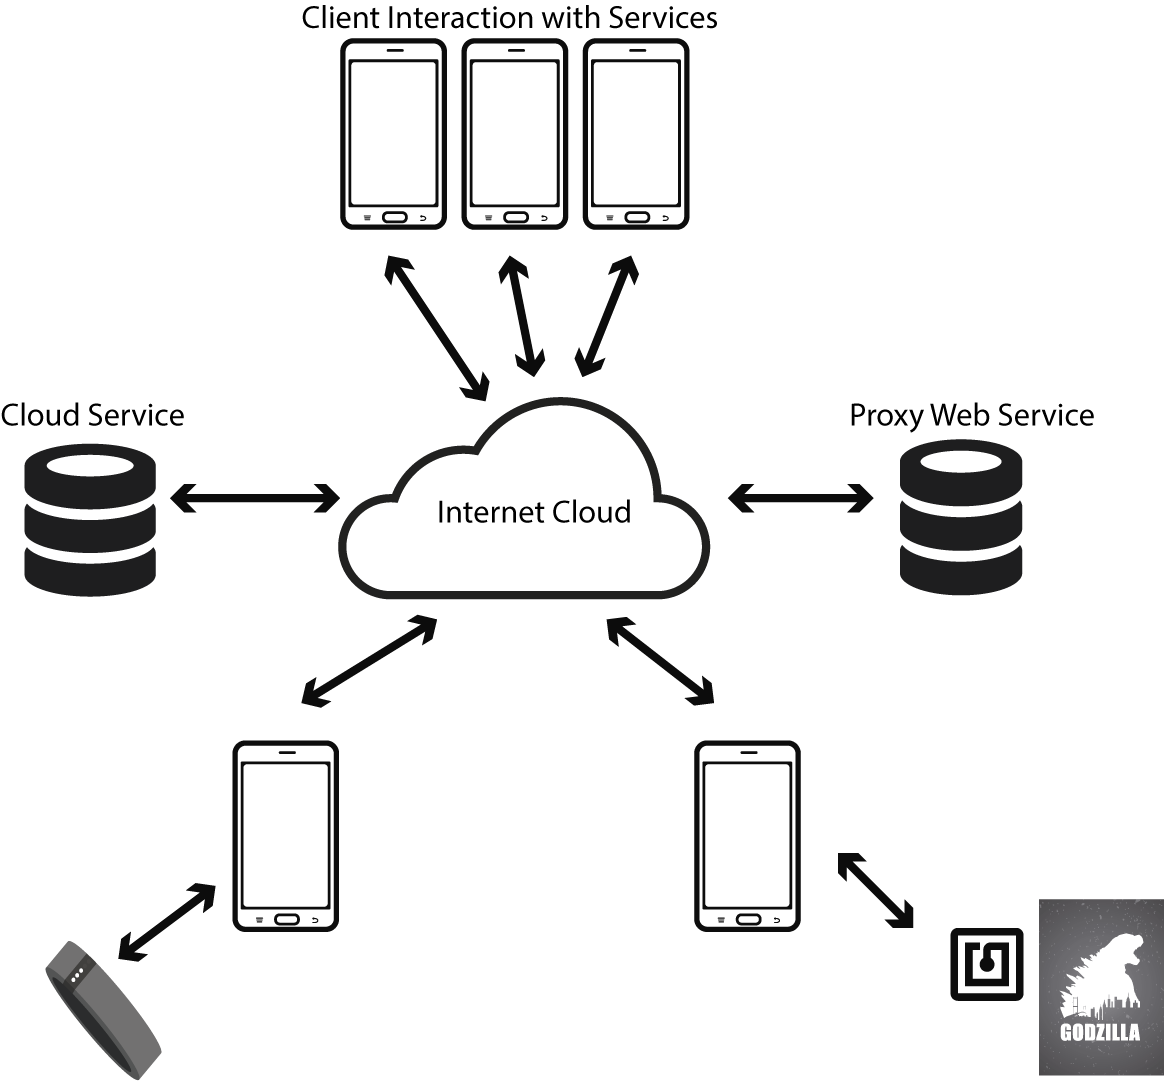
\includegraphics[width=0.6\textwidth]{graphs/ImagenTFG}
		\end{center}
		\caption{Ejemplos de comunicaci�n cercana}
	\end{figure}
	En la Web F�sica, personas, lugares y objetos tienen p�ginas web que proveen informaci�n y mecanismos de interacci�n. Sin embargo, es la amplitud y la profundidad de la pila que rodea a la web, que hacen de esta una atractiva visi�n para la evoluci�n del \ac{IOT}.\cite{enablingInternetThings}
	\\
	Las p�ginas web son una fant�stica tecnolog�a para interacci�n \ac{H2M}, pero muchos de los casos de uso del \ac{IOT} son interacciones \ac{M2M}. Los formatos de datos usados por \url{Schema.org} y otros, permiten a los agentes de usuario y servicios en la nube analizar los datos para eventos, organizaciones, personas, lugares, productos y as� sucesivamente, acutando sobre ellos de forma interactiva y proactiva.  \cite{enablingInternetThings}
	\\
	Uno de los primeros proyectos en fomentar esta idea fue \ac{HP} con \textit{Cooltown}, que usaba balizas infrarrojas para transmitir URLs. M�s recientemente, \ac{BLE} proporciona una similar baliza de bajo consumo que puede emitir \ac{URL} en paquetes peri�dicos (\url{www.uribeacon.org}). \cite{enablingInternetThings}
	\\
	
	\subsection*{Redes inal�mbricas e internet de las cosas}
	
	El futuro de internet tiene como meta integrar diferentes tecnolog�as de comunicaci�n, cableadas e inal�mbricas, con el objetivo de contribuir sustancialmente a mejorar el concepto de \ac{IOT} \cite{smartObjectBlock}. Aunque hay muchas maneras de describir el \ac{IOT}, podemos definirlo como una red con objetos interconectados con direcciones �nicas, basadas en un protocolo est�ndar de comunicaci�n.\cite{evolutionWirelesSensorNetworks}
	\\
	Los sensores de bajo costo han facilitado la proliferaci�n de \ac{WSN} en muchos escenarios como monitorizaci�n medioambiental, agricultura, salud, y construcciones inteligentes. \ac{WSN} est�n caracterizadas por una alta heterogeneidad porque est�n basadas en diferentes soluciones, propietarias y no propietarias. Este gran rango de soluciones est� retrasando actualmente desarrollos a gran escala de estas tecnolog�as a fin de que se obtenga una gran red virtual de sensores que permita integrar todos las existentes redes de sensores.\cite{fromTodayFutureInternet}
	\\
	%TODO a�adir imagen  "Interworking among heterogeneous WSNs. " de la cita: fromTodayFutureInternet
	Las redes de sensores basadas en sistemas cerrados o propietarios son islas conectivamente hablando, con limitadas comunicaciones con el mundo exterior. Por lo general, es necesario usar \textit{gateways} con conocimiento espec�fico de la aplicaci�n para exportar los datos de la \ac{WSN} a otros dispositivos conectados a Internet. Adem�s, no hay comuniaci�n directa entre diferentes protocolos a menos que se implementen complejas conversiones espec�ficas para la aplicaci�n en los \textit{gateways} o \textit{proxies}.
	
	\subsubsection*{Visi�n general de las soluciones existentes}
	En este apartado presentaremos una r�pida visi�n general de las principales tecnolog�as usadas para \ac{WSN} \cite{wirelessAutomationNetworks}. Analizaremos las soluciones que no est�n basadas en los protocolos de internet. 
	
	\paragraph{ZIGBEE} 
	ZigBee es una tecnolog�a de red inal�mbrica desarrollada por la ZigBee Alliance para baja tasa de transmisi�n de datos y aplicaciones de corto alcance \cite{ZigBeeHome}. La pila de protocolos ZigBee  est� compuesta por 4 principales capas: la capa \ac{PHY}, la capa \ac{MAC}, la capa \ac{NWK} y la capa \ac{APL}. \ac{PHY} y \ac{MAC} de ZigBee est�n definidas por el est�ndar \ac{IEEE} 802.15.4, mientras el resto de la pila est� definida por la especificaci�n ZigBee.
	\\
	Esta versi�n inicial del \ac{IEEE} 802.15.4, en la que ZigBee est� basado, funciona en la bandas de 868 MHz (Europa), 915 MHz (Norteam�rica) y 2.4 GHz (global).
	\\
	Una nueva especificaci�n de ZigBee es RF4CE \cite{ZigBeeRF4C}, que tiene una simplificada pila de red para topolog�as en estrellas solamente, ofreciendo una soluci�n simple para el control remoto de electr�nica de consumo.
	
	\paragraph{Z-WAVE} Z-Wave es un protocolo inal�mbrico desarrollado por ZenSys y promovida por la Z-Wave Alliance para automatizaciones residenciales y peque�os entornos comerciales. El principal objetivo de permitir transmisiones seguras de cortos mensajes desde una unidad de control hasta uno m�s nodos en la red \cite{ZWaveProtocol}. Z-Wave esta organizado de acuerdo a un arquitectura cumpuesta por 5 capas principales: \ac{PHY}, \ac{MAC}, transferencia, enrutado y capas de aplicaci�n.
	\\
	Z-Wave opera principalmente en la banda de 900 MHz (868 MHz en Europa y 908 MHz en Estados Unidos) y 2.4 GHz. Z-Wave permite tasas de transmisi�n a 9.6 kb/s, 40 kb/s y 200 kb/s.
	
	\paragraph{INSTEON}
	INSTEON \cite{InsteonDetails} es una soluci�n desarrollada por SmartLabs y promovida por la INSTEON Alliance. Una de las distintivas caracter�sticas de INSTEON es el hecho de como define una topolog�a de red compuesta de \ac{RF} y \textit{power line links}. Los dispositivos pueden ser \ac{RF},  \textit{power-line}, o pueden soportar ambos tipos de comunicaci�n.
	\\
	INSTEON opera a 904 MHz como frecuencia central, con una tasa de datos bruta de 38.4 kb/s.
	\\
	Los dispositivos INSTEON son parejas, lo que significa que cualquiera de ellos pueden tener el rol de emisor, receptor o repetidor. La comunicaci�n entre ambos dispositivos que no est�n en el mismo rango se logra mediante un enfoque <<multisalto>> que usa los repetidores en un esquema de sincronizaci�n temporal.
	
	\paragraph{WAVENIS}
	Wavenis es un protocolo inal�mbrico desarrollado por Coronis System para el control y monitorizaci�n de aplicaciones en entornos exigentes, incluida la dom�tica y la automatizaci�n de edificios. Wavenis actualmente est� promovida y gestionada por la \ac{Wavenis-OSA}. Est� definido por la funcionalidad de las capas f�sica, de enlace y de red \cite{ProblemSolvingWireless}. Los servicios de Wavenis pueden ser accedidos desde capas superiores mediante una \ac{API}.
	\\
	Wavenis opera principalmente en las bandas de 433 MHz, 868 MHz y 915 MHz, que son bandas reservadas para \ac{ISM} en Asia, Europa y Estados Unidos. Algunos productos tambi�n operan en la banda de 2.4 GHz. Las tasas de transmisi�n m�nimas y m�ximas dadas por Wavenis son 4.8 kb/s y 100 kb/s, respectivamente, con 19.2 kb/s como valor t�pico.
	
	\paragraph{TI 15.4-STACK}
	
	

\sectionx{Metodolog�a y directrices seguidas}
	
	
	
\sectionx{Estructura del documento}


	
\sectionx{�mbito de aplicaci�n}
	
	
\chapterend
%\part{Desarrollo del proyecto}

% Cap�tulo 01.
%%%%%%%%%%%%%%%%%%%%%%%%%%%%%%%%%%%%%%%%%%%%%%%%%%%%%%%%%%%%%%%%%%%%
%%% Documento LaTeX 																						%%%
%%%%%%%%%%%%%%%%%%%%%%%%%%%%%%%%%%%%%%%%%%%%%%%%%%%%%%%%%%%%%%%%%%%
% T�tulo:		Cap�tulo 1
% Autor:  	Ignacio Moreno Doblas
% Fecha:  	2014-02-01
% Versi�n:	0.5.0
%%%%%%%%%%%%%%%%%%%%%%%%%%%%%%%%%%%%%%%%%%%%%%%%%%%%%%%%%%%%%%%%%%%
\chapterbegin{Manual b�sico de \LaTeX}
\label{chp:ManLaTeX}
\minitoc

\begin{sinopsis}
\label{sec:chpltx:sinop}
	�ste es el primer cap�tulo de desarrollo del proyecto, definido y estructurado seg�n el autor necesite y desee. \nli
	En este caso, no hay gu�as gen�ricas para cualquier proyecto m�s all� del manual de estilo comentado anteriormente.

	En esta plantilla, este cap�tulo se enfoca como un manual b�sico de \LaTeX\ para cualquiera que lo necesite.
	
	Como plantilla, est� basada en la \ttw{\textbackslash documentclass} tipo \ttw{book}, empleando partes, cap�tulos, secciones, etc.\nli
	Quiz� para un proyecto fin de carrera no sean necesarias varias partes, as� que el autor puede suprimirlas si quiere.
	
	\LaTeX\ es una herramienta muy orientada a documentos que contienen tablas, figuras, referencias cruzadas, bibliograf�a, glosarios, ap�ndices, ecuaciones matem�ticas o unidades f�sicas.
\end{sinopsis}

\section{Estructura y formato del proyecto}
\label{sec:EstrForm}
	Esta plantilla sigue las especificaciones de la ETSIT para presentar un TFG/PFC/TFM. \nli
	Igualmente, la plantilla con su material adicional est� disponible en la \tit{web} del centro (\url{www.etsit.uma.es}.)

\section{Apartados de la plantilla}
	La plantilla est� estructurada en los siguientes archivos y directorios:
\begin{itemize}
	\item{Veintid�s ficheros \TeX\ (extensi�n \ttw{.tex}).}
	
	\item{Un fichero Bib\TeX\ (extensi�n \ttw{.bib}).}
	
	\item{Un fichero PDF resultante.}
	
	\item{Dos ficheros \TeX nicCenter (extensi�n \ttw{.tps} y \ttw{.tcp}).}
	
	\item{Dos directorios complementarios.\nli
		Uno de c�digo fuente (\ttw{code}) y otro de gr�ficos (\ttw{graphs}).}
	
\end{itemize}

	En la figura~\ref{fig:ficherosPlan}, puede verse la lista de ficheros del proyecto, tal y como se presenta en el entorno \TeX nicCenter.

	A su vez, los veintid�s ficheros \TeX\ contienen un documento maestro a partir del cual se referencia el resto de archivos, repartidos en cuatro clases.
	
	Los archivos contienen un prefijo que hace que su posici�n en la lista sea equivalente al orden en el documento PDF resultante. Este prefijo es una letra y un n�mero en ar�bigo. 
	
	Por ejemplo, el documento maestro, ``\ttw{A0.Mi Proyecto fin de carrera.tex}'' comienza por \ttw{A0} para que figure en primer lugar.

	Las cuatro clases de archivos antes mencionadas son las siguientes:
\begin{descript}
	\item[Archivos de pre�mbulo]{Forman el pre�mbulo del documento \LaTeX\ y su contenido no se visualiza en el fichero PDF resultante.\nli
		Comienzan por la letra \ttw{A} y un n�mero desde el uno al cuatro.}
	\item[Archivos iniciales]{Son los archivos iniciales del proyecto, desde la portada, si la hay, dedicatoria, acr�nimos, tablas de contenido, pr�logo e introducci�n.\nli
		Comienzan por la letra \ttw{B} y un n�mero del cuatro al siete.}
	\item[Archivos de cap�tulo]{Son los ficheros de cap�tulo del proyecto.\nli
	Dado que su primera letra coincide con la letra C, no tienen ninguna identificaci�n especial.}
	\item[Archivos finales]{Por �ltimo, los archivos de conclusiones, ap�ndices, bibliograf�a y glosario (\tit{index} en ingl�s).}
\end{descript}

\begin{figure}[h]
	\centering
		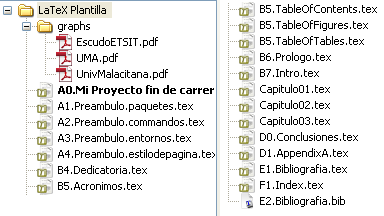
\includegraphics[width=9cm]{graphs/ArchivosPlantilla.png}
	\caption{Ficheros de la plantilla}
	\label{fig:ficherosPlan}
\end{figure}

	En la figura~\ref{fig:ficherosPlan}, segmentada en dos mitades, se observan todos estos archivos ordenados seg�n el orden secuencial como se visualiza en el documento PDF.\nli
	Esta ordenaci�n permite una elaboraci�n c�moda del proyecto en sus diferentes secciones. Se recomienda mantener esta ordenaci�n.\nli
	Por contra, si no se hubieran creado los prefijos, los ap�ndices aparecer�an en el entorno antes que los cap�tulos, aunque en el PDF ocurra al rev�s. Esta distribuci�n har�a m�s dif�cil para el proyectando producir un documento ordenado y limpio.
	
	\medskip
	En el documento PDF resultante, el proyecto se estructura en los nueve apartados siguientes:
\begin{descript}
	\item[Portada y encuadernaci�n.]{Es espec�fica de cada tipo de trabajo (TFG/PFC/TFM) y debe ajustarse a lo establecido en la Secretar�a.
	
	Para esta plantilla, s�lo en el caso de los PFC del plan a extinguir se provee de una portada. Para los TFG y TFM, existen plantillas externas que pueden descargarse de la \tit{web} de la ETSIT.}

	\item[Primeras p�ginas.]{Contendr� las p�ginas que correspondan con el tipo de trabajo y que es espec�fica de cada tipo de proyecto.}
	
	\item[Agradecimientos y dedicatoria.]{La secci�n de agradecimientos (evidentemente, no obligatoria) define un apartado donde el proyectando puede (y quiz�s, debe) referenciar a aquellas personas y/o instituciones que, de manera generosa, han colaborado de alg�n modo en la gestaci�n y desarrollo del PFC.\nli
	Igualmente el proyectando tambi�n puede utilizar este apartado libremente para mencionar a aquellos familiares, compa�eros, amigos, etc., de los que ha recibido apoyo personal, moral o afectivo.\nli
	Por contra, no debe utilizarse esta secci�n para expresar opiniones cr�ticas, �cidas o mordaces contra particulares o instituciones de la ETSIT o la Universidad debido a correcciones, ex�menes, trato recibido u otras interacciones o causas cualesquiera que sean.\nli
	Estar�a fuera del �mbito del proyecto y debe respetarse.
}
	
	\item[�ndice.]{En la plantilla, se genera un �ndice, �ndice de figuras e �ndice de tablas, numerado autom�ticamente con su correspondiente p�gina. �sta es una de las ventajas de \LaTeX.}
	
	\item[Cap�tulo de Introducci�n.]{En �ste se har� una introducci�n al �mbito del trabajo, comenzando por el contexto general y aproxim�ndose progresivamente a los aspectos m�s concretos que se traten. \nli
	Es conveniente terminar con una exposici�n clara de los objetivos que se persiguen, la metodolog�a empleada y el contenido del proyecto.}
	
	\item[Cap�tulos de desarrollo.]{A continuaci�n el desarrollo de los distintos cap�tulos o ep�grafes que componen el trabajo.\nli
	En esta plantilla, �ste es ese cap�tulo, que adem�s incluye un manual de \LaTeX\ pr�ctico.}
	
	\item[Conclusiones.]{En este apartado el estudiante expondr� con claridad los resultados o conclusiones obtenidas y el juicio cr�tico que le merecen.}
	
	\item[Referencias bibliogr�ficas.]{A continuaci�n de las conclusiones se insertar�n un apartado con todas las referencias bibliogr�ficas que aparezcan en la memoria: revistas, art�culos de revistas o congresos, p�ginas web, etc.
	
	En \LaTeX, existe el entorno Bib\TeX\ para almacenar y referenciar bibliograf�a.}
	
	\item[Ap�ndices.]{Finalmente se presentar�n los ap�ndices, si los hubiere.
	
	En esta plantilla se provee del entorno \ttw{\textbackslash appendix} para crearlos.}
\end{descript}

	Por �ltimo, respecto de las secciones del proyecto, hay que tener en cuenta que un proyecto puede ser un documento extenso, complejo y por eso se recomienda seguir este tipo de reglas para facilitar su elaboraci�n.\nli
	Adem�s, se recomienda generarlo incrementalmente, anulando las secciones que no se utilicen desde el documento maestro. Por ejemplo, al elaborar el cap�tulo tres y generar el documento PDF, no es necesario ni el pr�logo, ni los cap�tulos anteriores ni posteriores, por tanto, pueden comentarse con el s�mbolo tanto por ciento (\ttw{\%}). En ese caso, la compilaci�n ser� m�s r�pida, el PDF m�s breve y la revisi�n tambi�n.

\section{Referencias Cruzadas}
\label{sec:RefCruz}
	Normalmente, surge la necesidad de referenciar informaci�n desde una secci�n de la documentaci�n hasta otra.\nli
	Esta informaci�n referenciada puede ser un apartado, una figura, una tabla, una p�gina o una ecuaci�n.
	
	Por ejemplo, el presente cap�tulo~\ref{chp:ManLaTeX} comienza en la p�gina~\pageref{chp:ManLaTeX} y est� titulado \nameref{chp:ManLaTeX}.\nli
	Tanto el n�mero de cap�tulo, su p�gina o su t�tulo no est�n escritos manualmente, sino referenciados mediante etiquetas.
	
	Las referencias cruzadas se realizan siguiendo tres pasos secuenciales:
\begin{enu}
	\item{Se etiqueta el elemento a referenciar, ya sea secci�n, apartado, figura, tabla, ecuaci�n o cualquier otro con el comando \ttw{\textbackslash label}.\nli
	Para ello, se escribe pr�ximo a �l un identificador con el comando \ttw{\textbackslash label}.\nli
	Por ejemplo, \ttw{\textbackslash label\{sec:RefCruz\}} es la etiqueta del presente apartado.\nli
	Se recomienda, en general, usar como prefijo \ttw{chp} para cap�tulos, \ttw{sec} para secciones, \ttw{eq} para ecuaciones, \ttw{fig} para figuras o \ttw{tab} para tablas. Tambi�n usar los dos puntos (:) como separador entre el prefijo y el resto de la etiqueta.\nli
	A lo largo de esta plantilla pueden encontrarse muchas etiquetas de ejemplo.}
	
	\item{Se compila si es la primera vez que se crea la etiqueta.
	Aunque este paso depende del compilador, en el caso de MiK\TeX\ es necesario compilar para indexar la etiqueta y poder referenciarla, como se indica en el paso siguiente.}

	\item{Se referencia una etiqueta ya definida con el comando \ttw{\textbackslash ref}.\nli
		Por ejemplo, \ttw{\textbackslash ref\{sec:RefCruz\}} referencia el presente apartado, cuyo valor es \ref{sec:RefCruz}.}
	
	\item{Se compila el documento para crear la referencia a partir de los �ndices generados en la compilaci�n anterior.\nli
	Esto es especialmente importante, porque la referencia se crea a partir de la compilaci�n anterior. Si el apartado cambia de p�gina, se debe re-compilar para actualizar la referencia; si no se compila, la referencia se har� seg�n la informaci�n desactualizada, es decir, a la p�gina anterior.\nli
	\emph{En general y t�rminos pr�cticos, se debe compilar frecuentemente para tener siempre informaci�n actualizada.}}
\end{enu}

%\section{Formato de otros elementos}
\section{Figuras}
	Las figuras aparecer�n centradas y se ver�n siempre acompa�adas por un t�tulo explicativo, tambi�n centrado y situado en la parte inferior.\nli	
	El t�tulo comienza por la palabra ``Figura'' con un identificador de figura formado por el n�mero de cap�tulo y el n�mero de figura.\nli
	El propio t�tulo debe ser lo bastante explicativo para poder entender el significado de la figura o distinguirla de las dem�s, pero no puede ser muy extenso para ser c�modamente legible.\nli
	Para cualquier explicaci�n o justificaci�n m�s extensa, se debe describir en un p�rrafo aparte, utilizando referencias cruzadas.
	%Por ejemplo, si se est�n mostrando resultados, el t�tulo ha describir brevemente en qu� condiciones se han obtenido los resultados mostrados.
	Adem�s, tanto el t�tulo como el identificador aparecer�n referenciados en el �ndice de figura al principio de la memoria.
	\smallskip
	
	En \LaTeX, el entorno \ttw{figure} automatiza la presentaci�n de figuras siguiendo estas reglas.\nli
	A continuaci�n se ve el texto original utilizado para la figura~\ref{fig:escudo:ETSIT} de la p�gina~\pageref{fig:escudo:ETSIT}, titulada \nameref{fig:escudo:ETSIT}.\nli
	Para respetar los espacios y el texto original se ha utilizado el entorno \ttw{lstlisting}.
	
\begin{lstlisting}
	\begin{figure}[h]
		\centering
		
\includegraphics[width=3cm]{graphs/EscudoETSIT.pdf}
		\caption{Escudo oficial de la ETSIT}
		\label{fig:escudo:ETSIT}
	\end{figure}
\end{lstlisting}

\begin{figure}[h]
	\centering
		
\includegraphics[width=3cm]{graphs/EscudoETSIT.pdf}
	\caption{Escudo oficial de la ETSIT}
	\label{fig:escudo:ETSIT}
\end{figure}

	\ \\[1ex]
	Puede ser necesario presentar una figura conteniendo varias en su interior. En ese caso, el entorno \ttw{\textbackslash minipage} cumple esta funci�n.\nli
	En la figura~\ref{fig:escudo:UMA}, se muestran los dos escudos de la Universidad de M�laga.
	
	\begin{figure}[h]
		\centering
			\begin{minipage}[l]{4cm}
			
\includegraphics[width=4cm]{graphs/UMA.pdf}
			\end{minipage}
			\ \ 
			\begin{minipage}[r]{4cm}
			
\includegraphics[width=4cm]{graphs/UnivMalacitana.pdf}
			\end{minipage}
		\caption{Escudos oficiales de la UMA}
		\label{fig:escudo:UMA}
	\end{figure}
	
	
	Tambi�n es importante conocer varias caracter�sticas sobre los gr�ficos vectoriales y pixelados (tambi�n llamados rasterizados\footnote{en ingl�s, \tit{raster}.}) y sobre los formatos aceptados por \LaTeX\ para gr�ficos, aunque esto depender� del compilador utilizado.

\smallskip
	
	En general, hay dos tipos de ficheros gr�ficos en un ordenador:
\begin{descript}
	\item[Pixelados o rasterizados]{El gr�fico est� formado por una matriz de p�xeles, como en una fotograf�a digital.\nli
	Ejemplos de formatos rasterizados son JPG, PNG, GIF o TIFF.}

	\item[Vectoriales]{El gr�fico est� formado por curvas geom�tricas, lo que hace que independientemente de la escala mostrada, se mantenga la misma definici�n, tanto en color como en forma.\nli
	Ejemplos de formatos vectoriales son EPS (\tit{Encapsulated PostScript}), PDF o SVG (\tit{Scalable Vector Graphics}).\nli
	Un ejemplo concreto es la figura~\ref{fig:escudo:ETSIT}, que est� en PDF.
	}
\end{descript}

	Las explicaciones siguientes est�n enfocadas al entorno de Windows MiK\TeX\ y \TeX nicCenter. Puede haber variaciones en otros entornos de \LaTeX\ como \TeX Live\ (usado en Linux) o \TeX shop (usado en Apple\R).

	Si se desea insertar un gr�fico vectorial y se emplea el compilador \ttw{pdflatex.exe} de MiK\TeX, el formato del gr�fico debe ser PDF.\nli	
	Si los gr�ficos vectoriales est�n en otro formato, tales como SVG o EPS, es necesario usar un conversor.\nli
	Una opci�n sencilla y gratuita es el editor Inkscape\R, disponible en Internet. No es necesario instalarlo, ya que puede encontrarse una edici�n portable, que s�lo requiere ser descomprimida y ejecutada.	

\section{Tablas}
	La presentaci�n de las tablas es equivalente a la de las figuras, tanto en su posici�n centrada como en su t�tulo.
	
	En \LaTeX\ existen varios entornos para presentar una tabla, dependiendo de qu� se desee:
	\begin{ite}
		\item{El entorno \tbf{\ttw{tabular}} permite crear una tabla a partir de definir sus filas, columnas y su formato.\nli
		Est� limitado a no poder fragmentarse en varias p�ginas si la tabla es demasiado extensa.}
		\item{El entorno \tbf{\ttw{table}} formatea una tabla, una secci�n de c�digo fuente o alg�n componente equivalente.\nli
		Permite posicionar, ponerle un t�tulo y a�adirlo al �ndice de tablas.\nli
		En el ejemplo siguiente, se utilizan los dos entornos, uno \ttw{table} y otro \ttw{tabular} anidado en el primero.}
		\item{El entorno \tbf{\ttw{longtable}} es equivalente a \ttw{tabular}, pero adem�s supera la limitaci�n de extender una tabla a m�s de una p�gina.}
	\end{ite}
	
	De nuevo, las tablas aparecen referenciadas en un �ndice de tablas tras el �ndice tem�tico y del �ndice de figuras.
	
	A continuaci�n, se muestra el c�digo \LaTeX\ de la tabla~\ref{tab:SAR}, presente en la p�gina~\ref{tab:SAR}, titulada \nameref{tab:SAR}.
	
\begin{lstlisting}
	\begin{table}[h]%
	\centering
	\begin{tabular}{|c|p{14ex}|c|c|}
		\hline
		\hline
		\tbf{Requisito} & \tbf{Plat. Ref.} & 
			\tbf{SAR (dBm)} & \tbf{Tol.}\\
		\hline
		R101  &  Baytrail & 5 & 1 \\
		\hline
		R201  &  Clovertrail & 6 & 2\\
		\hline
		R301  &  Merrifield & 4 & 3\\
		\hline
		\hline
	\end{tabular}
	\caption{Tabla de SAR por Plat. de Ref.}
	\label{tab:SAR}
	\end{table}
\end{lstlisting}
	
	%\begin{center}
	\begin{table}[h]%
	\centering
	%\begin{longtable}{c|p{10cm}}
	\begin{tabular}{|c|p{14ex}|c|c|}
		\hline
		\hline
		\tbf{Requisito} & \tbf{Plat. Ref.} & \tbf{SAR (dBm)} & \tbf{Tol.}\\
		\hline
		R101  &  Baytrail & 5 & 1 \\
		\hline
		R201	&	 Clovertrail & 6 & 2\\
		\hline
		R301	&  Merrifield & 4 & 3\\
		\hline
		\hline
	\end{tabular}
	\caption{Tabla de SAR por Plat. de Ref.}
	\label{tab:SAR}
	\end{table}
	%\end{longtable}
	%\end{center}%\end{table}

\section{C�digo fuente}
	En un proyecto de desarrollo, es com�n introducir extractos de c�digo en diferentes lenguajes como C, C++, Matlab, Python, Java, bash script, etc.\nli
	En estos casos, los entornos de \LaTeX\ disponibles por defecto no permiten mostrar esta informaci�n.
	
	El paquete \ttw{listings} permite presentar c�digo fuente, respetando las tabulaciones para que la lectura sea confortable.
	
	En esta plantilla, en la secci�n de paquetes se ha configurado c�digo Python para presentar los ejemplos. Es f�cilmente adaptable para otros lenguajes.\nli
	En la secci�n de comandos, se dispone del comando \ttw{code} que permite crear una secci�n de c�digo indicando el t�tulo a mostrar, el fichero fuente correspondiente y la etiqueta con la que se har�n referencias.
	
	A continuaci�n, se muestra un ejemplo:
	
\begin{verbatim}
	\code{C�digo Python de ejemplo}{code/pythonCode.py}{code:python}
\end{verbatim}

\code{C�digo Python de ejemplo}{code/pythonCode.py}{code:python}

	Una limitaci�n importante del paquete \ttw{listings} es que no resalta las palabras reservadas del lenguaje ni otros elementos, una caracter�stica muy deseable para el lector.
	
	Para eso, existe otro paquete \LaTeX\ m�s reciente, \ttw{minted}, disponible en \cite{minted}\footnote{\url{https://code.google.com/p/minted/}}.

\section{S�mbolos matem�ticos y f�sicos}
	Los proyectos de ingenier�a suelen presentar s�mbolos matem�ticos y f�sicos, tanto en los p�rrafos como en tablas, figuras y ecuaciones.
	
	Existen reglas para la notaci�n, formateo y estilo de elementos matem�ticos, tales como utilizar un s�mbolo por variable (p.ej., $x$ e $y$, pero no $xx$ o $yy$), escribir los s�mbolos en cursiva y las magnitudes y unidades f�sicas en redonda o el espaciado entre variables.
	
	\LaTeX\ est� construido sobre \TeX, que fue concebido originalmente para escribir textos matem�ticos con alta calidad, de forma que funciona perfectamente en estos entornos. Su integraci�n es suave, r�pida y sencilla de seguir, una vez se tiene algo de pr�ctica.
	
	Una extensi�n de esto es el uso de magnitudes f�sicas con sus correspondientes m�ltiplos. En \LaTeX\ se provee del paquete \ttw{SIunits}, presente en esta plantilla.
	
	A continuaci�n se muestran varios ejemplos de su uso, con su c�digo original.

	Para ecuaciones integradas en el p�rrafo, tan s�lo se usa el s�mbolo d�lar (\$) antes y despu�s del s�mbolo. Por ejemplo, con \$\tit{\ttw{x}}\$ se indica la variable $x$.\nli
	Las ecuaciones en l�nea deben usarse limitadamente. Para escribir ecuaciones m�s largas est�n los entornos \ttw{displaymath}, \ttw{equation} y \ttw{align}.
	\smallskip
	
	Los entornos \ttw{displaymath} y \ttw{equation} muestran una ecuaci�n en una l�nea. La diferencia entre ambos es que el primero no realiza una numeraci�n de la ecuaci�n y el segundo s�. S�lo se puede hacer una referencia a una ecuaci�n numerada.
	
	Por ejemplo, la ecuaci�n de la proporci�n �urea en entorno \ttw{displaymath},
\begin{lstlisting}
	\begin{displaymath}
		\phi^2 - \phi - 1 = 0
	\end{displaymath}
\end{lstlisting}

\begin{displaymath}
	\phi^2 - \phi - 1 = 0
\end{displaymath}

y en entorno \ttw{equation}, mostrando la ecuaci�n~\ref{eq:aurea} en la p�gina~\pageref{eq:aurea}:
\begin{lstlisting}
	\begin{equation}
		\phi^2 - \phi - 1 = 0
		\label{eq:aurea}
	\end{equation}
\end{lstlisting}

\begin{equation}
	\phi^2 - \phi - 1 = 0
	\label{eq:aurea}
\end{equation}

%\begin{equation}
	%\int_0^\infty \mathrm{e}^{-x}\,\mathrm{d}x = z
	%\label{eq:prueba}
%\end{equation}

	En caso de querer desarrollar una ecuaci�n en varias l�neas, se debe emplear el entorno \ttw{align}. Funciona como un entorno \ttw{array} de dos columnas separadas por el s�mbolo d�lar.\nli
	Por ejemplo, el desarrollo en serie de Fourier de una funci�n $x(t)$ en forma trigonom�trica y exponencial,
\begin{align}
	x(t) & = \frac{a_0}{2} %\\
	     + \sum_{k = 1}^{k = \infty}{A_k \cos(\omega_{k} t)}
			 + \sum_{k = 1}^{k = \infty}{B_k \sin(\omega_{k} t)}\label{eq:fou:trig} \\
			 & = \sum_{k = -\infty}^{k = \infty}{X_k e^{j \omega_k t}}\label{eq:fou:exp}
\end{align}

	Referenciando ambas ecuaciones, la ecuaci�n~\ref{eq:fou:trig} desarrolla la serie de Fourier de forma trigonom�trica y la ecuaci�n~\ref{eq:fou:exp} de forma exponencial.
	
	En caso de no querer mostrar ninguna numeraci�n en las ecuaciones, se debe usar el entorno \ttw{align*}.
	
	En caso de querer desarrollar una ecuaci�n, pero s�lo numerar algunas de ellas, se debe a�adir el comando \ttw{\textbackslash nonumber} a las ecuaciones que no deseen ser numeradas.

	Como anotaci�n, existe tambi�n el entorno \ttw{eqnarray}, pero presenta limitaciones, tales como referenciar varias ecuaciones dentro de un entorno. Por esta raz�n es mejor usar el entorno \ttw{align}.
	
	Respecto a las magnitudes y unidades f�sicas, la tabla~\ref{tab:ctes} (p�g.~\pageref{tab:ctes}) muestra diferentes constantes f�sicas.

\begin{table}[h]
\centering
\begin{tabular}{p{8cm}cp{3cm}}
	\hline
	Constante Gravitacional & $G_0$ & $6.67 \, 10^{-11} \, \newton\metre^2\per\kilogram^2$\\
	Constante de Planck & $h$ & $6.63 \, 10^{-34} \, \joule\cdot\second$\\
	Constante de Stefan-Boltzman & $\sigma$ & $5.67 \, 10^{-8} \watt\per\metre^2\kelvin^4$\\
	Carga elemental & $e$ & $1.6 \cdot 10^{-19} \, \coulomb$\\
	Masa del electr�n & $m_e$ & $9.11 \, 10^{-31} \kilogram$\\
	Velocidad de la luz en el vac�o & $c_0$ & $3 \, 10^8 \metre\per\second$ \\
	Permitividad el�ctrica en el vac�o & $\epsilon_0$ & $8.85 \, 10^{-12} \, \farad\per\metre$\\
	Permeabilidad magn�tica en el vac�o & $\mu$ & $1.26 \, 10^{-6} \, \henry\per\metre$\\
	\hline
\end{tabular}
	\caption{Constantes f�sicas (usando \ttw{SIunits})}
	\label{tab:ctes}
\end{table}

	En el manual de \ttw{SIunits}, presente en un PDF entre el material adicional adjunto a esta plantilla, se puede encontrar el resto de magnitudes y unidades a utilizar (especialmente, p�g.~25 y sigs.).

\section{Referencias bibliogr�ficas}
	Adem�s del etiquetado de secciones, tablas, figuras y ecuaciones a lo largo del proyecto, debe referenciarse el origen bibliogr�fico de todos los datos necesarios.
	
	Para eso, \LaTeX\ incluye la herramienta Bib\TeX, que permite almacenar fuentes bibliogr�ficas (libros, art�culos, revistas, p�ginas web, seminarios, etc.) en un archivo y formato est�ndar, referenciarlas mediante etiquetas (equivalente a las referencias a secciones, tablas, figuras y ecuaciones) y variar el estilo bibliogr�fico seg�n se prefiera.
	En esta plantilla se incluyen dos ficheros,
\begin{ite}
	\item{\ttw{E2.Bibliografia.bib}. Fichero que contiene todas las fuentes bibliogr�ficas utilizando la estructura de Bib\TeX.}
	\item{\ttw{E1.Bibliografia.tex}. Fichero que al final de la memoria que imprime las referencias seg�n el estilo bibliogr�fico seleccionado entre varias opciones. Tambi�n incluye la referencia a la bibliograf�a en la Tabla de contenidos del proyecto.}
\end{ite}

	Respecto al estilo bibliogr�fico, el autor puede seleccionar el que considere mejor seg�n su criterio.\nli
	Bib\TeX\ ofrece los siguientes estilos bibliogr�ficos:
\begin{descript}
	\item[plain]{Es el estilo b�sico (de ah�, su nombre). Las entradas se ordenan alfab�ticamente y se etiquetan con un n�mero (p.ej., [1])}
	\item[unsrt]{Es igual que plain, pero aparecen en orden de citaci�n.}
	\item[alpha]{El etiquetado se hace por autor y a�o de publicaci�n (p.ej., [Knu66])}
	\item[abbrv]{Igual que alpha, pero m�s abreviado.}
\end{descript}
	
	Comparando esta plantilla con la gu�a de estilo (v�ase~\cite{GuiaEstilo}, p�g. 13 y sigs.), los estilos \ttw{plain} y \ttw{unsrt} corresponden con el denominado m�todo num�rico y los estilos \ttw{alpha} y \ttw{abbrv} con el m�todo autor y a�o.

\section{Formato de los Ap�ndices}
	Se incluye en los ap�ndices informaci�n complementaria al texto del proyecto que no se considera indispensable para su compresi�n.
	
	Ejemplo: Ap�ndice A: M�todos de generaci�n de ruidos gaussianos fraccionarios.

	Los ap�ndices se numeran alfab�ticamente y para su redacci�n, se han de seguir las reglas de seccionado como en los cap�tulos anteriores, no tiene ninguna peculiaridad.

\section{Glosario de t�rminos}
	Un glosario (en ingl�s, \tit{index}) referencia palabras importantes dentro del documento y la p�gina o p�ginas en que puede encontrarse este t�rmino.

	En \LaTeX, la herramienta \ttw{MakeIndex} presente en el paquete \ttw{makeidx} se encarga de gestionar los ap�ndices. Esta plantilla lo incluye.
	
	Aunque \ttw{MakeIndex} ofrece muchas m�s prestaciones, se muestra un uso b�sico con el comando \ttw{\textbackslash miindex}. Con �l se crea la palabra seleccionada y se inserta con su referencia a p�gina.

\section{Sobre los correctores ortogr�ficos}
	\LaTeX\ no incluye un corrector ortogr�fico como Microsoft Word\R.\nli
	Tampoco el compilador de Windows\R MiK\TeX, que s�lo recibe un fichero fuente en formato TXT y lo entrega en PDF.
	
	Si se desea esta funcionalidad\footnote{Es muy recomendable, en mi opini�n (Nota del autor).}, se depende del entorno de desarrollo. En este caso, esta plantilla est� hecha en \TeX nicCenter, que incluye un diccionario de palabras a corregir.
	
	A pesar de eso, se incluye un diccionario en espa�ol que debe instalarse seg�n las notas indicadas en el fichero l�ame.

\section{Dec�logo del usuario novel de \LaTeX}
	Como se ha comentado anteriormente, la curva de aprendizaje de \LaTeX\ es dif�cil\footnote{A�n as�, es justo decir que conseguir un documento de equivalente calidad no resulta mucho m�s f�cil en otro sistema, ya que requiere conocer funciones avanzadas.}, as� que se recomienda seguir estas recomendaciones:
\begin{enumerate}
	\item{S� pr�ctico, aprende lo que necesites para el proyecto de esta plantilla y util�zalo.}
	\item{Sigue la plantilla, est� pensada para proveerte de todo lo necesario.}
	\item{Usa formularios (en ingl�s, \tit{cheat sheet}) y busca en internet lo que necesites.}
	\item{Cuanto antes, inst�late un entorno \LaTeX\ (un MiK\TeX y un \TeX nicCenter, por ejemplo) y practica con �l.}
	\item{Practica con el entorno, especialmente el \tit{debugueo}.}
	\item{S� paciente, deja que \LaTeX\ te resulte familiar.}
	\item{Si despu�s de intentarlo, no lo consigues, no lo uses, no es obligatorio. No te castigues.}
	\item{No te conviertas en tip�grafo, no profundices demasiado.}
	\item{Busca ayuda como en Cervan\TeX\footnote{\url{www.cervantex.es}}. Tienen una lista de correo activa y te contestar�n.}
	\item{Deja el estilo para el final.}
	
\end{enumerate}


\section{Otras recomendaciones}
	Finalmente, hay cuatro recomendaciones a tener en cuenta durante la redacci�n del proyecto. Son consejos pr�cticos basados en la experiencia que resultar�n �tiles.
\begin{descript}
	\item[Ficheros de compilaci�n.]{El compilador MiK\TeX\ genera ficheros de salida tales como el resultado de la compilaci�n (los \tit{logs}), muy importantes en caso de tener que encontrar causas de origen en un fallo; tablas de contenido, tablas de figuras, ficheros que realimentan la siguiente compilaci�n como las referencias cruzadas, o la bibliograf�a.\nli
	Como recomendaci�n, mantener estos ficheros actualizados y utilizar las opciones del entorno de desarrollo para borrarlos o guardarlos en una ubicaci�n espec�fica.}
	
	\item[Codificaci�n de archivos]{Existen varios formatos de codificaci�n de archivos, que condicionan c�mo los ceros y unos representan los caracteres. \nli
	Por ejemplo, ANSI o UTF-8.\nli
	Dependiendo del formato, el compilador puede malinterpretar los caracteres, generando un documento err�neo, t�picamente con los acentos. A veces, incluso, el lector puede leer bien el texto pero el compilador no, siendo m�s dif�cil detectar este hecho. La causa es que el editor de texto tiene reglas diferentes del compilador \LaTeX. Tambi�n es com�n que ocurra esto en un situaci�n de copiar y pegar texto.\nli
	En ese caso, debe cambiarse la codificaci�n para que sea correcta. Una forma sencilla de hacerlo en Windows\R\ es utilizando el Notepad++. Hay una opci�n de codificaci�n.}
	
	\item[Referenciar a ficheros]{Para la referencia a ficheros en figuras o a c�digo fuente, hay que usar ficheros. Es recomendable que su nombre tenga un juego de caracteres reducido, es decir, alfanum�rico y poco m�s, y que su ruta de acceso siga esa regla tambi�n, es decir, en los directorios relativos respecto del directorio principal.\nli
	Por ejemplo, en esta plantilla, las gr�ficas est�n en el directorio `code' y los gr�ficos en el directorio `graphs'.}
	
	\item[Cervan\TeX.]{El grupo espa�ol de usuarios de \LaTeX\ se llama Cervan\TeX. Su p�gina web es \url{www.cervantex.es}. Disponen de una lista de distribuci�n en la que se pueden preguntar dudas.\nli
	Es muy recomendable tenerla en cuenta.}
\end{descript}

\chapterend{}

% Cap�tulo 02.
%%%%%%%%%%%%%%%%%%%%%%%%%%%%%%%%%%%%%%%%%%%%%%%%%%%%%%%%%%%%%%%%%%%%
%%% Documento LaTeX 																						%%%
%%%%%%%%%%%%%%%%%%%%%%%%%%%%%%%%%%%%%%%%%%%%%%%%%%%%%%%%%%%%%%%%%%%
% T�tulo:		Cap�tulo 2
% Autor:  	Ignacio Moreno Doblas
% Fecha:  	2014-02-01
% Versi�n:	0.5.0
%%%%%%%%%%%%%%%%%%%%%%%%%%%%%%%%%%%%%%%%%%%%%%%%%%%%%%%%%%%%%%%%%%%
\chapterbegin{T�tulo del cap�tulo}
\label{chp:Utiliz}
%\minitoc

\section{T�tulo del apartado}
\label{sec:TestSuiteCrec}

\section{T�tulo del apartado}



\chapterend{}

% Cap�tulo 03.
%%%%%%%%%%%%%%%%%%%%%%%%%%%%%%%%%%%%%%%%%%%%%%%%%%%%%%%%%%%%%%%%%%%%
%%% Documento LaTeX 																						%%%
%%%%%%%%%%%%%%%%%%%%%%%%%%%%%%%%%%%%%%%%%%%%%%%%%%%%%%%%%%%%%%%%%%%
% T�tulo:		Cap�tulo 3
% Autor:  	Ignacio Moreno Doblas
% Fecha:  	2014-02-01
% Versi�n:	0.5.0
%%%%%%%%%%%%%%%%%%%%%%%%%%%%%%%%%%%%%%%%%%%%%%%%%%%%%%%%%%%%%%%%%%%
\chapterbegin{T�tulo del cap�tulo}
\label{chp:App}
%\minitoc

%\section{Nombre de la sección}
%
%\section{Nombre de la sección}
%
%\section{Nombre de la sección}


\chapterend{}

% Cap�tulo 04.
%\input{Capitulo04.tex}


%\part{Pruebas y funcionamiento}

%\part{Conclusiones y lineas futuras}
%\chapterbeginx{Conclusiones y l�neas futuras}

\sectionx{Conclusiones}
	Despu�s de todo el desarrollo del proyecto, es pertinente hacer una valoraci�n final del mismo, respecto a los resultados obtenidos, las expectativas o el resultado de la experiencia acumulada.

	En esta secci�n se exponen todos esos conceptos y enuncian unas conclusiones finales.
	
	Adem�s, considerando tambi�n el estado de la t�cnica, se pueden deducir l�neas futuras de trabajo, proponer otros puntos de vista o cualquier otra sugerencia como post�mbulo del presente trabajo, para ser considerada por el lector o el tribunal evaluador.

\sectionx{L�neas futuras}

\begin{flushright}
{\large \pfcauthorname}\nli
\today
\end{flushright}
	
\chapterend

% Anexos
%\part{Ap�ndices}

%\appendix

%\pagestyle{fancy}
\fancyhead[LE,RO]{\thepage}
\fancyhead[RE]{Ap�ndice} %
\fancyhead[LO]{\nouppercase{\rightmark}}
%\fancyhead[RE]{Parte \thepart \rightmark} %

\chapter{Estructuras de mensajes OTA}
\label{apd:estructurasMensajes}

Em la figura \ref{fig:mensajesSMSGS} se observan los distintos tipos de mensajes que se env�an sobre la red inal�mbrica, estos mensajes est�n definidos en el fichero \textit{smsgs.h}

\begin{figure}[H]
	\centering
	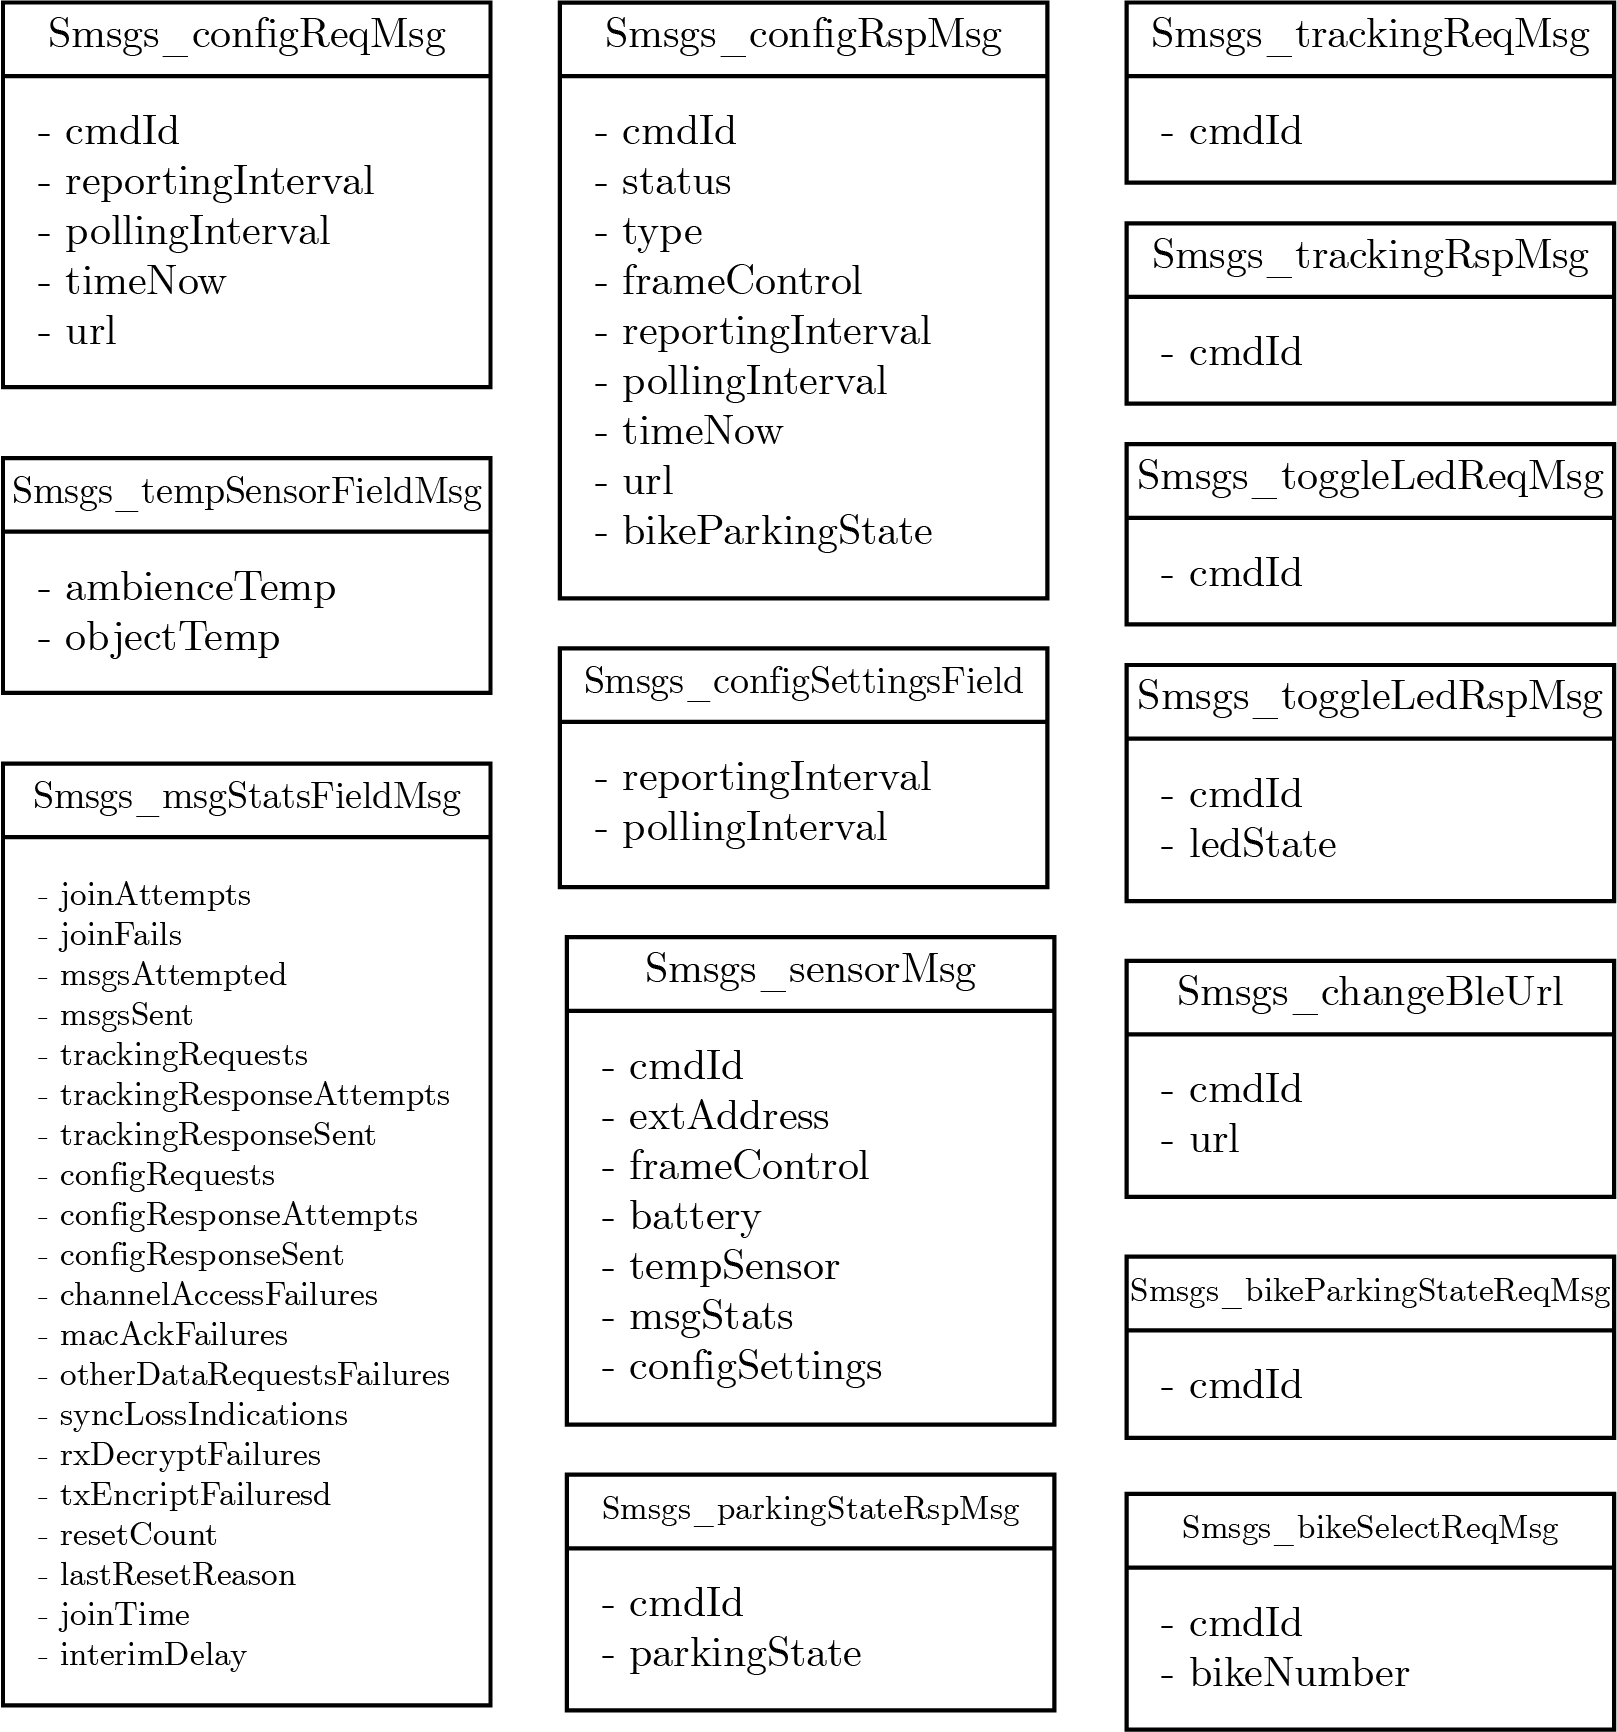
\includegraphics[width=\textwidth]{graphs/mensajesSMSGS}
	\caption{Estructuras de los mensajes del fichero smsgs.h}
	\label{fig:mensajesSMSGS}
\end{figure}


%\pagestyle{fancy}
\fancyhead[LE,RO]{\thepage}
\fancyhead[RE]{Ap�ndice} %
\fancyhead[LO]{\nouppercase{\rightmark}}
%\fancyhead[RE]{Parte \thepart \rightmark} %

\chapter{Herramientas utilizadas}
\label{apd:herramientasUtilizadas}

\begin{center}
	\begin{longtable}{ m{0.3\textwidth} p{0.7\textwidth} }
		
\includegraphics[align=t,width=0.2\textwidth]{graphs/logo-github}& 
		GitHub es una plataforma para alojar proyectos utilizando el sistema de control de versiones GIT.
		\\ 
		\hline
		 
\includegraphics[align=t,width=0.2\textwidth]{graphs/logo-aws} &  
		 \textit{Amazon Web Services} (AWS) es una colecci�n de servicios web que conjunto forman una plataforma de computaci�n en la nube.
		  \\ 
		  \hline
		   
\includegraphics[align=t,width=0.2\textwidth]{graphs/logo-texStudio} &  
		  TeXstudio es un entorno de escritura intregrado para crear documentos LaTeX.
		  \\ 
		  \hline
		  
		  
\includegraphics[align=t,width=0.2\textwidth]{graphs/logo-latex} &  
		  LaTeX es un sistema de composici�n de textos, orientado a la creaci�n de documentos escritos que presenten una alta calidad tipogr�fica.
		  \\ 
		  \hline
		  
		  
\includegraphics[align=t,width=0.2\textwidth]{graphs/logo-illustrator} &  
		  Adobe Illustrator es un editor de gr�ficos vectoriales y est� destinado a la creaci�n art�stica de dibujo y pintura para ilustraci�n. 
		  \\ 
		  \hline
		  
		  
\includegraphics[align=t,width=0.2\textwidth]{graphs/logo-sublime} &  
		  Sublime text es un editor de texto y editor de c�digo fuente.
		  \\ 
		  \hline
		  
		  
\includegraphics[align=t,width=0.2\textwidth]{graphs/logo-node} &  
		  Node.js es un entrono de ejecuci�n para JavaScript construido con el motor de JavaScript V8 de Chrome. 
		  \\ 
		  \hline
		  
		  
\includegraphics[align=t,width=0.2\textwidth]{graphs/logo-angular} &  
		  AngularJS es un \textit{framework} de JavaScript de c�digo abierto, mantenido por Google, que se utiliza para crear y mantener aplicaciones web de una sola p�gina.
		  \\ 
		  \hline
		  
		  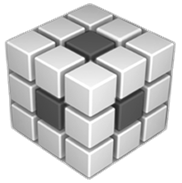
\includegraphics[align=t,width=0.2\textwidth]{graphs/logo-ccs} &  
		  Code Composer Studio es un entorno integrado de desarrollo que soporta los microcontroladores de Texas Instruments. 
		  \\ 
		  \hline
		  
		  
\includegraphics[align=t,width=0.2\textwidth]{graphs/logo-mongo} &  
		  MongoDB es una base de datos NoSQL orientado a documentos, desarrollado bajo el concepto de c�digo abierto.
		  \\ 
		  \hline
		  
		  
\includegraphics[align=t,width=0.2\textwidth]{graphs/logo-raspbian} &  
		  Raspbian es un distribuci�n del sistema operativo GNU/Linux y basado en Debian Jessie para la Raspberry Pi.
		  \\ 
		  \hline
		  
		  
\includegraphics[align=t,width=0.2\textwidth]{graphs/logo-express} &  
		  Express es una infraestructura de aplicaciones web Node.js m�nima y flexible que proporciona un conjunto s�lido de caracter�sticas para las aplicaciones web y m�viles.
		  \\ 
		  \hline

	\end{longtable} 
\end{center}

\chapterend

%\input{D3.AppendixC.tex}

% Formato de documento en la parte final.
\backmatter
%Hace que los cap�tulos y t�tulos nivel inferior no aparezcan numerados (lo que es ideal para conclusiones o notas finales).

% Bibliograf�a
%%%%%%%%%%%%%%%%%%%%%%%%%%%%%%%%%%%%%%%%%%%%%%%%%%%%%%%%%%%%%%%%%%%
%%% Documento LaTeX 																						%%%
%%%%%%%%%%%%%%%%%%%%%%%%%%%%%%%%%%%%%%%%%%%%%%%%%%%%%%%%%%%%%%%%%%%
% T�tulo:		Bibliograf�a
% Autor:  	Ignacio Moreno Doblas
% Fecha:  	2014-02-01
% Versi�n:	0.5.0
%%%%%%%%%%%%%%%%%%%%%%%%%%%%%%%%%%%%%%%%%%%%%%%%%%%%%%%%%%%%%%%%%%%%

% Encabezamiento %
\pagestyle{fancy}
\fancyhead[LE,RO]{\thepage}
\fancyhead[LO]{Bibliograf�a}
%\fancyhead[RE]{Parte \thepart \rightmark} %
\fancyhead[RE]{\nouppercase{\rightmark}} %

%Inclusi�n de bibliograf�a%
\bibliography{E2.Bibliografia} %�sese el nombre del fichero sin extensi�n

%Inclusi�n en el �ndice (Tabla de contenidos)
\addcontentsline{toc}{chapter}{Bibliograf�a}

%Formateo de estilo de bibliograf�a
% Otros formatos: plain, unsrt, abbrv
%  plain: las entradas se ordenan alfab�ticamente y se etiquetan con un n�mero (p.ej., [1])
% unsrt: igual que plain, pero aparecen en orden de citaci�n.
% alpha: el etiquetado se hace por autor y a�o de publicaci�n (p.ej., [Knu66]).
% abbrv: igual que alpha, pero m�s abreviado.
\bibliographystyle{alpha}

%Impresi�n de todas las entradas bibliogr�ficas
\nocite{*}

\chapterend

% �ndice alfab�tico%
%%%%%%%%%%%%%%%%%%%%%%%%%%%%%%%%%%%%%%%%%%%%%%%%%%%%%%%%%%%%%%%%%%%
%%% Documento LaTeX 																						%%%
%%%%%%%%%%%%%%%%%%%%%%%%%%%%%%%%%%%%%%%%%%%%%%%%%%%%%%%%%%%%%%%%%%%
% T�tulo:		Glosario (index)
% Autor:  	Ignacio Moreno Doblas
% Fecha:  	2014-02-01
% Versi�n:	0.5.0
%%%%%%%%%%%%%%%%%%%%%%%%%%%%%%%%%%%%%%%%%%%%%%%%%%%%%%%%%%%%%%%%%%%%

\pagestyle{fancy}
\fancyhead[LE,RO]{\thepage}
\fancyhead[LO]{�ndice Alfab�tico}
%\fancyhead[RE]{Parte \thepart \rightmark} %
\fancyhead[RE]{\nouppercase{\rightmark}} %

%index of contents
\phantomsection
\addcontentsline{toc}{chapter}{�ndice alfab�tico}
\printindex


%Example 	Index Entry 	Comment
%\index{hello} 	hello, 1 	Plain entry
%\index{hello!Peter} 	  Peter, 3 	Subentry under 'hello'
%\index{Sam@\textsl{Sam}} 	Sam, 2 	Formatted entry
%\index{Lin@\textbf{Lin}} 	Lin, 7 	Same as above
%\index{Jenny|textbf} 	Jenny, 3 	Formatted page number
%\index{Joe|textit} 	Joe, 5 	Same as above
%\index{ecole@\'ecole} 	�cole, 4 	Handling of accents
%\index{Peter|see{hello}} 	Peter, see hello 	Cross-references
%\index{Jen|seealso{Jenny}} 	Jen, see also Jenny 	Same as above

\chapterend

\end{document}